\documentclass[uplatex, dvipdfmx, a4paper, twocolumn]{jsarticle}
\usepackage[dvipdfm, margin=20mm]{geometry}
\usepackage{flushend}
\usepackage{fancyhdr}
\pagestyle{fancy}
\lhead{}
\chead{\small 島田 : 自然言語処理parser試作に関する報告書}
\rhead{}
\renewcommand{\headrulewidth}{0pt}

\usepackage{mathtools}
\usepackage{siunitx}
\sisetup{detect-all}
\usepackage{url}
\usepackage[normalem]{ulem}
%\usepackage{censor}
%\StopCensoring

\usepackage{graphicx}
\usepackage{subfig}
\captionsetup{
  format=hang,
  labelsep=quad,
  labelfont=bf,
  font=small,
}
%\usepackage{here}
\usepackage[monochrome]{xcolor}
\usepackage{gnuplot-lua-tikz}

\usepackage{newtxtext}
\usepackage{newtxmath}
%\usepackage[T1]{fontenc}
%\usepackage{lmodern}
%\usepackage{libertine}

\usepackage{docmute}
\usepackage{titling}
\usepackage[addtotoc]{abstract}
%\usepackage[
%  backend=biber,
%  sorting=none,
%]{biblatex}
%\addbibresource{mybib.bib}
\usepackage[super, sort&compress]{natbib}
\bibpunct{}{)}{,}{s}{}{\textsuperscript{,}}
\renewcommand{\bibnumfmt}[1]{#1)}
\bibliographystyle{unsrt}
\renewcommand{\refname}{参考文献}
\makeatletter
\def\thefootnote{\ifnum\c@footnote>\z@\leavevmode\lower.5ex\hbox{$\ast$}\@arabic\c@footnote\fi}
\makeatother
%\renewcommand{\thefootnote}{$\ast$\arabic{footnote}}
\newcommand\fig[1]{\textbf{図\ref{#1}}}
\newcommand\tab[1]{\textbf{表\ref{#1}}}
\newcommand\refsec[1]{\textsf{\ref{#1}}}

\usepackage[
  pdftitle={自然言語処理parser試作に関する報告書},
  pdfauthor={島田 歩},
  pdfborder={0 0 0},
]{hyperref}
\usepackage{pxjahyper}
\usepackage{listings,jlisting}
\lstset{
  language={C},
  basicstyle={\small\ttfamily},
  frame={tb},
  numbers=left,
  xleftmargin=3zw,
  numberstyle={\scriptsize},
  lineskip=-0.5ex,
  breaklines=true,
}
\usepackage{fancyvrb}
\usepackage{tikz-qtree}

\begin{document}
  \thispagestyle{empty}
  \twocolumn[
    \emptythanks
    \title{
      %\protect\\ 
      \hspace{0.3zw}自然言語処理parser試作に関する報告書\addtocounter{footnote}{-1}\thanks{2017年12月1日 仮提出 ; 2017年12月6日 受理 ;}
      \addtocounter{footnote}{-1}\thanks{2017年12月12日 更新}
    }
    \author{
      島田 歩
      \rlap{\normalfont\textsuperscript{\dag}}
    }
    \date{
      \itshape\small
      {\normalfont\textsuperscript{\dag}}ayumu.shimada@gmail.com
    }

    {
      \let\newpage\relax
      \renewcommand\thispagestyle[1]{\relax}
      %\renewcommand\footnotemark{}
      \maketitle
    }
  ]\saythanks

  \section{始めに}\label{hajimeni}
  本実験報告書は以下の章立てで構成されている:
  \begin{description}
    \item[\autoref{hajimeni}] 始めに
    \item[\autoref{mokuteki}] 実験の目的
    \item[\autoref{gaiyou}] 自然言語処理の概要
    \item[\autoref{kekka}] 実験の結果
    \item[\autoref{kousatu}] 考察
    \item[\autoref{matome}] まとめ
  \end{description}
  また,巻末には,参考文献リストと付録および手書きの図がある.

  特に,\autoref{kousatu}の考察では,文の解釈を一意に特定できない問題と非文が生成される問題について述べている.

  \section{実験の目的}\label{mokuteki}
  自然言語処理において,基本技術の一つになっている構文解析技法について,その原理を学ぶ\cite{jikken3c1}.
  また,自然言語処理における構文解析の困難さについても実際に体験する.

  \section{自然言語処理の概要}\label{gaiyou}
  自然言語処理(natural language processing: NLP)とは,人間が書いたり話したりしたりする文章をコンピュータに処理させることである\cite{jikken3c1}.
  これは,文章の中の単語の品詞を決定するための形態素解析,単語間のつながりを調べる構文解析,単語や文の意味を解析する意味解析および必要な応答文を生成する等の処理を含む\cite{jikken3c1}.

  また,Chomskyによれば,言語は,形式言語を用いて階層化できる(\autoref{fig:chomsky}).
  なお,正規文法は有限オートマトンで,文脈自由文法(context-free grammar: CFG)はプッシュダウンオートマトンで,それぞれ認識できる.
  \begin{figure}[htpb]
    \centering
    \resizebox{0.9\linewidth}{!}{
      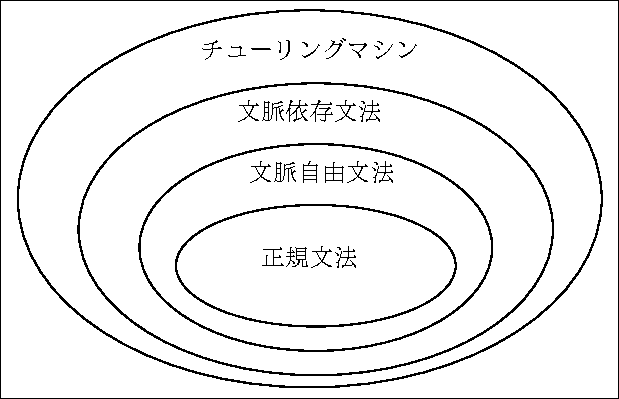
\includegraphics{fig/chomsky.pdf}
    }
    \caption{Chomskyの言語階層\cite{jikken3c1}}
    \label{fig:chomsky}
  \end{figure}

    \subsection{有限オートマトン}
    有限オートマトンは入力記号列と現在の状態に応じて次の状態へ遷移する.
    入力記号列を入力し終えたときに受理状態にあれば,その入力記号列は受理可能である.

    \subsection{プッシュダウンオートマトン}
    有限オートマトンに補助記憶装置としてプッシュダウンスタックを取り付けたものがプッシュダウンオートマトンである.
    入力記号列を入力し終えたときに受理状態にあり,かつ,スタックが空であれば,その入力記号列は受理可能である.

    \subsection{あいまい性}
    文脈自由文法では,構文木が複数得られることがある.
    この場合,その文法はあいまいであると言う.

  \section{実験の結果}\label{kekka}
    \subsection{ネットワーク文法の実験}
      \subsubsection{手による解析}
      \autoref{tab:syntax_network}の文法規則と\autoref{tab:dict_girl_network}の単語辞書を用いて
      ``I saw a girl with a telescope .''を形態素解析した結果を\textbf{図~\addtocounter{figure}{1}\thefigure}に示す.
      \begin{table}[htb]
        \centering
        \caption{ネットワーク文法の文法規則\cite{jikken3c1}}
        \label{tab:syntax_network}
        \begin{tabular}{l c l} \hline
          start & $\to$ & DET (冠詞) \\
          start & $\to$ & NOUN (名詞) \\
          DET (冠詞) & $\to$ & NOUN (名詞) \\
          DET (冠詞) & $\to$ & ADJ (形容詞) \\
          DET (冠詞) & $\to$ & NOUN (名詞) \\
          ADJ (形容詞) & $\to$ & NOUN (名詞) \\
          NOUN (名詞) & $\to$ & PREP (前置詞) \\
          PREP (前置詞) & $\to$ & NOUN (名詞) \\
          PREP (前置詞) & $\to$ & ADJ (形容詞) \\
          PREP (前置詞) & $\to$ & DET (冠詞) \\
          NOUN (名詞) & $\to$ & VERB (動詞) \\
          VERB (動詞) & $\to$ & ADV (副詞) \\
          VERB (動詞) & $\to$ & DET (冠詞) \\
          ADV (副詞) & $\to$ & PREP (前置詞) \\
          NOUN (名詞) & $\to$ & ADV (副詞) \\
          ADV (副詞) & $\to$ & NOUN (名詞) \\
          VERB (動詞) & $\to$ & end \\
          NOUN (名詞) & $\to$ & end \\ \hline
        \end{tabular}
      \end{table}
      \begin{table}[htb]
        \centering
        \caption{``I saw a girl with a telescope.''の単語辞書}
        \label{tab:dict_girl_network}
        \begin{tabular}{l c l} \hline
          I & $\to$ & NOUN (名詞) \\
          saw & $\to$ & VERB (動詞) \\
          a & $\to$ & DET (冠詞) \\
          girl & $\to$ & NOUN (名詞) \\
          with & $\to$ & PREP (前置詞) \\
          telescope & $\to$ & NOUN (名詞) \\
          . & $\to$ & end \\ \hline
        \end{tabular}
      \end{table}
      \begin{table}[htb]
        \centering
        \caption{``the child runs quickly to the large house.''の単語辞書}
        \label{tab:dict_child_network}
        \begin{tabular}{l c l} \hline
          the & $\to$ & DET (冠詞) \\
          child & $\to$ & NOUN (名詞) \\
          runs & $\to$ & VERB (動詞) \\
          quickly & $\to$ & ADV (副詞) \\
          to & $\to$ & PREP (前置詞) \\
          large & $\to$ & ADJ (形容詞) \\
          house & $\to$ & NOUN (名詞) \\
          . & $\to$ & end \\ \hline
        \end{tabular}
      \end{table}

      \subsubsection{プログラムによる解析}
      文法規則と単語辞書に\autoref{tab:syntax_network}, \autoref{tab:dict_girl_network}および\autoref{tab:dict_child_network}を用い,
      作成したプログラムで``I saw a girl with a telescope .''と``the child runs quickly to the large house .''の2文を形態素解析した結果を示す.
      \begin{figure*}[htpb]
        \centering
        %\resizebox{0.9\linewidth}{!}{
        \fbox{
          \BVerbatimInput{fig/result_network.txt}
        }
        \caption{プログラムによる形態素解析結果}
        \label{fig:result_network}
      \end{figure*}

    \subsection{文脈自由文法の実験}
      \subsubsection{手による解析}
      \autoref{tab:syntax_girl}の文法規則と\autoref{tab:dict_girl_network}の単語辞書を用いて
      top-down法およびCYK法により構文解析した結果を,
      それぞれ\textbf{図~\addtocounter{figure}{1}\thefigure}, \textbf{図~\addtocounter{figure}{1}\thefigure}に示す.
      \begin{table*}[htb]
        \centering
        \caption{``I saw a girl with a telescope''の文法規則}
        \label{tab:syntax_girl}
        \begin{tabular}{l c l c l} \hline
          S (文) & $\to$ & NP (名詞句) & $+$ & VP (動詞句) \\
          NP (名詞句) & $\to$ & NOUN (名詞) & & \\
          NP (名詞句) & $\to$ & DET (冠詞) & $+$ & NOUN (名詞) \\
          VP (動詞句) & $\to$ & VERB (動詞) & & \\
          VP (動詞句) & $\to$ & VERB (動詞) & $+$ & NP (名詞句) \\
          VP (動詞句) & $\to$ & VERB (動詞) & $+$ & SS \\
          SS & $\to$ & NP (名詞句) & $+$ & PP (前置詞句) \\
          PP (前置詞句) & $\to$ & PREP (前置詞) & $+$ & NP (名詞句) \\ \hline
        \end{tabular}
      \end{table*}

      \subsubsection{プログラムによる解析}
      \autoref{tab:syntax_child}の文法規則と\autoref{tab:dict_child_network}の単語辞書を用い,
      作成したプログラムで``the child runs quickly to the large house''をCYK法により構文解析した結果得られた構文木とS式をそれぞれ
      \autoref{fig:tree_child}と\autoref{fig:result_cyk}に示す.
      \begin{table*}[htb]
        \centering
        \caption{``the child runs quickly to the large house''の文法規則}
        \label{tab:syntax_child}
        \begin{tabular}{l c l c l} \hline
          S (文) & $\to$ & NP (名詞句) & $+$ & VP (動詞句) \\
          NP (名詞句) & $\to$ & DET (冠詞) & $+$ & NOUN (名詞) \\
          NP (名詞句) & $\to$ & DET (冠詞) & $+$ & NP (名詞句) \\
          NP (名詞句) & $\to$ & PREP (前置詞) & $+$ & NP (名詞句) \\
          NP (名詞句) & $\to$ & ADJ (形容詞) & $+$ & NOUN (名詞) \\
          VP (動詞句) & $\to$ & VERB (動詞) & $+$ & NP (名詞句) \\
          VP (動詞句) & $\to$ & VPa (動詞句) & $+$ & NP (名詞句) \\
          VP (動詞句) & $\to$ & VERB (動詞) & $+$ & ADV (副詞) \\
          VP (動詞句) & $\to$ & VERB (動詞) & & \\
          VPa (動詞句) & $\to$ & VERB (動詞) & $+$ & ADV (副詞) \\
          VPa (動詞句) & $\to$ & VERB (動詞) & $+$ & NP (名詞句) \\ \hline
        \end{tabular}
      \end{table*}
      \begin{figure}[htpb]
        \centering
        \resizebox{0.95\linewidth}{!}{
          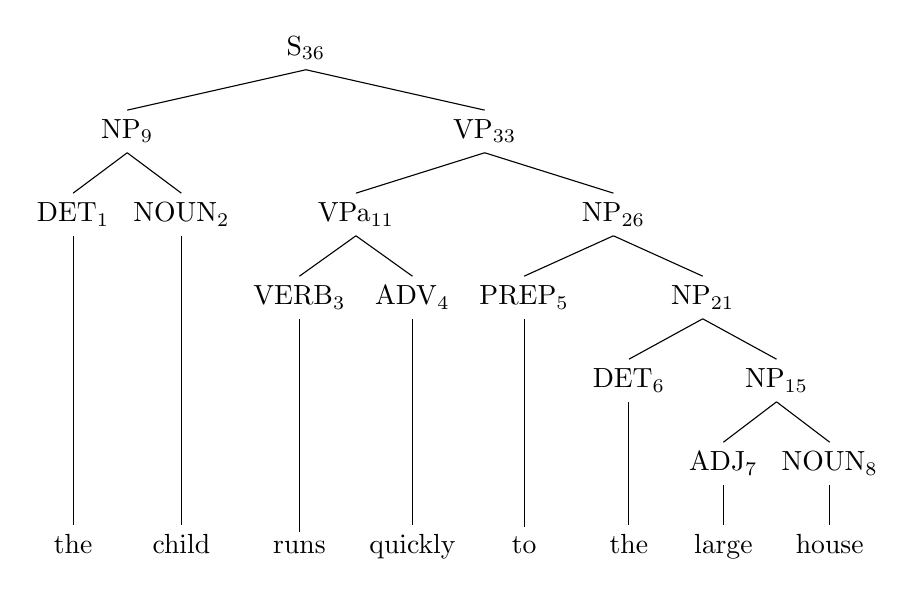
\begin{tikzpicture}
  \tikzset{frontier/.style={distance from root=180pt}}
  \Tree [.$\mathrm{S}_{36}$ [.$\mathrm{NP}_{9}$ [.$\mathrm{DET}_{1}$ the ] [.$\mathrm{NOUN}_{2}$ child ] ]
        [.$\mathrm{VP}_{33}$ [.$\mathrm{VPa}_{11}$ [.$\mathrm{VERB}_{3}$ runs ] [.$\mathrm{ADV}_{4}$ quickly ] ]
        [.$\mathrm{NP}_{26}$ [.$\mathrm{PREP}_{5}$ to ] [.$\mathrm{NP}_{21}$ [.$\mathrm{DET}_{6}$ the ]
        [.$\mathrm{NP}_{15}$ [.$\mathrm{ADJ}_{7}$ large ] [.$\mathrm{NOUN}_{8}$ house ] ] ] ] ] ]
\end{tikzpicture}

        }
        \caption{``the child runs quickly to the large house''の構文木}
        \label{fig:tree_child}      
      \end{figure}

      さらに,\autoref{tab:syntax_girl}の文法規則と\autoref{tab:dict_girl_network}の単語辞書を用い,
      ``I saw a girl with a telescope''を構文解析した結果得られた構文木とS式をそれぞれ
      \autoref{fig:tree_girl}と\autoref{fig:result_cyk}に示す.
      \begin{figure*}[htpb]
        \centering
        %\resizebox{0.9\linewidth}{!}{
        \fbox{
          \BVerbatimInput{fig/result_cyk.txt}
        }
        \caption{プログラムによる構文解析結果(印刷の関係上,出力は改行している.)}
        \label{fig:result_cyk}
      \end{figure*}

  \section{考察}\label{kousatu}
    \subsection{``I saw a girl with a telescope.''の2つの解釈}
    ``I saw a girl with a telescope.''には大きくわけて,以下の2つの意味(解釈)がある:
    \begin{itemize}
      \item 私は望遠鏡を持った少女に会った.(\autoref{fig:tree_girl})
      \item 私は望遠鏡で少女を見た.(\autoref{fig:tree_telescope})
    \end{itemize}
    今回の実験の結果得られた解釈は前者だが,\autoref{tab:syntax_girl}の文法規則に\(\text{VP} \to \text{VP} + \text{PP}\)を追加することにより,
    後者の解釈となる構文木(\autoref{fig:tree_telescope})とS式(\autoref{fig:result_telescope})が得られる.
    \begin{figure*}[htpb]
      \centering
      \subfloat[私は望遠鏡を持った少女に会った.]{
        \label{fig:tree_girl}
        \resizebox{0.45\linewidth}{!}{
          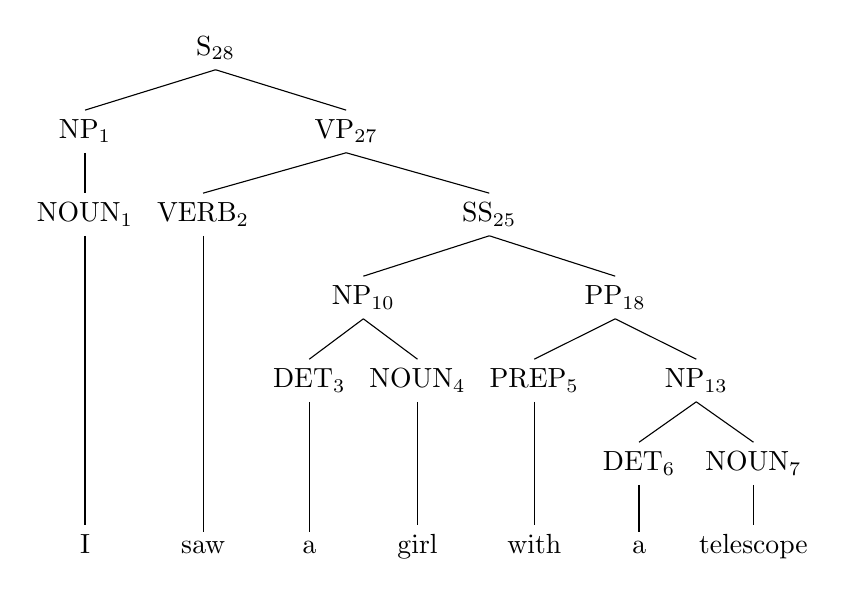
\begin{tikzpicture}
  \tikzset{frontier/.style={distance from root=180pt}}
  \Tree [.$\mathrm{S}_{28}$ [.$\mathrm{NP}_{1}$ [.$\mathrm{NOUN}_{1}$ I ] ] [.$\mathrm{VP}_{27}$ [.$\mathrm{VERB}_{2}$ saw ]
        [.$\mathrm{SS}_{25}$ [.$\mathrm{NP}_{10}$ [.$\mathrm{DET}_{3}$ a ] [.$\mathrm{NOUN}_{4}$ girl ] ]
        [.$\mathrm{PP}_{18}$ [.$\mathrm{PREP}_{5}$ with ] [.$\mathrm{NP}_{13}$ [.$\mathrm{DET}_{6}$ a ] [.$\mathrm{NOUN}_{7}$ telescope ] ] ] ] ] ]
\end{tikzpicture}

        }
      }
      \subfloat[私は望遠鏡で少女を見た.]{
        \label{fig:tree_telescope}
        \resizebox{0.45\linewidth}{!}{
          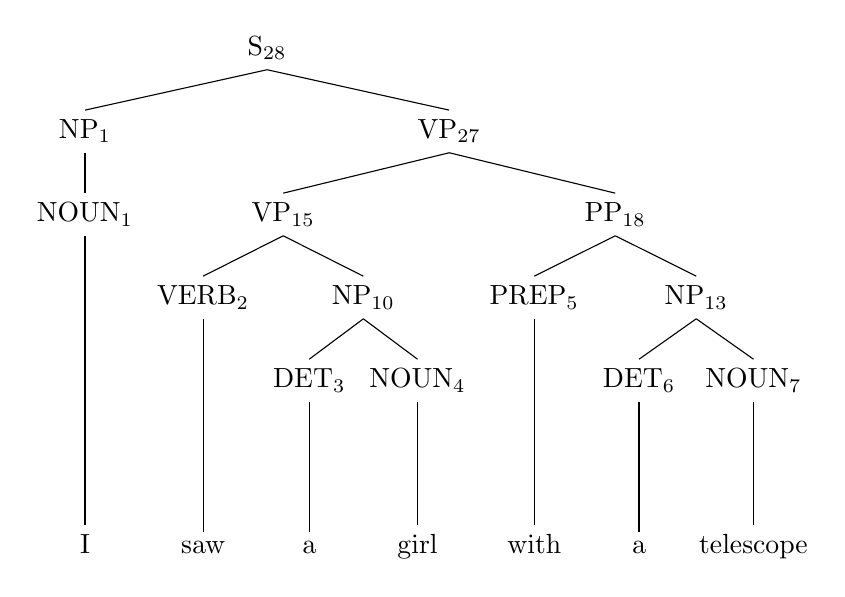
\begin{tikzpicture}
  \tikzset{frontier/.style={distance from root=180pt}}
  \Tree [.$\mathrm{S}_{28}$ [.$\mathrm{NP}_{1}$ [.$\mathrm{NOUN}_{1}$ I ] ] [.$\mathrm{VP}_{27}$ [.$\mathrm{VP}_{15}$
        [.$\mathrm{VERB}_{2}$ saw ] [.$\mathrm{NP}_{10}$ [.$\mathrm{DET}_{3}$ a ] [.$\mathrm{NOUN}_{4}$ girl ] ] ]
        [.$\mathrm{PP}_{18}$ [.$\mathrm{PREP}_{5}$ with ] [.$\mathrm{NP}_{13}$ [.$\mathrm{DET}_{6}$ a ] [.$\mathrm{NOUN}_{7}$ telescope ] ] ] ] ]
\end{tikzpicture}

        }
      }
      \caption{``I saw a girl with a telescope''の構文木}
    \end{figure*}
    \begin{figure*}[htpb]
      \centering
      %\resizebox{0.9\linewidth}{!}{
      \fbox{
        \BVerbatimInput{fig/result_telescope.txt}
      }
      \caption{私は望遠鏡で少女を見た(\autoref{fig:tree_telescope})という解釈になるS式(印刷の関係上,出力は改行している.)}
      \label{fig:result_telescope}
    \end{figure*}

    なお,複数のS式を得るためには,合致する文法規則を見つけるとそこで中止して次のセルに移動するような実装では不可能で,
    必ず全ての文法規則についてチェックを行い,合致する文法規則を全て記憶しておく必要がある.
    本プログラムはそれを考慮した実装になっているため,複数のS式が出力可能である.

    しかしながら,複数のS式が出力されるということは文の解釈を一意に特定できないということであり,この問題の解決は困難であると考えられる.

    \subsection{``Time flies like an arrow.''の解釈}
    \autoref{tab:syntax_flies}の文法規則と\autoref{tab:dict_flies}の単語辞書を用い
    ``Time flies like an arrow''を構文解析した結果,4つの構文木(\autoref{fig:tree_flies})とS式(\autoref{fig:result_flies})が得られた.
    これらの解釈はそれぞれ以下である:
    \begin{itemize}
      \item 時は矢のように過ぎる. $\Rightarrow$ 光陰矢のごとし.(\autoref{fig:tree_flies_1})
      \item time fly(トキバエ?)たちは矢を好む.(\autoref{fig:tree_flies_2})
      \item ``矢のようなハエ''たちの速度を測定せよ.(\autoref{fig:tree_flies_3})
      \item 矢(の速度を測定するとき)のように,ハエたちの速度を測定せよ.(\autoref{fig:tree_flies_4})
    \end{itemize}
    さらに,``Time''が雑誌の名前である可能性も考慮すると,さらに別の解釈も可能である.

    \begin{table}[htb]
      \centering
      \caption{``Time flies like an arrow''の文法規則}
      \label{tab:syntax_flies}
      \begin{tabular}{l c l c l} \hline
        S & $\to$ & NP & $+$ & VP \\
        S & $\to$ & VP & & \\
        NP & $\to$ & NOUN & & \\
        NP & $\to$ & DET & $+$ & NOUN \\
        NP & $\to$ & NOUN & $+$ & NP \\
        NP & $\to$ & NP & $+$ & PP \\
        VP & $\to$ & VERB & & \\
        VP & $\to$ & VERB & $+$ & NP \\
        VP & $\to$ & VP & $+$ & PP \\
        PP & $\to$ & PREP & $+$ & NP \\ \hline
      \end{tabular}
    \end{table}
    \begin{table}[htb]
      \centering
      \caption{``Time flies like an arrow''の単語辞書}
      \label{tab:dict_flies}
      \begin{tabular}{l c l} \hline
        Time & $\to$ & NOUN \\
        Time & $\to$ & VERB \\
        flies & $\to$ & NOUN \\
        flies & $\to$ & VERB \\
        like & $\to$ & PREP \\
        like & $\to$ & VERB \\
        an & $\to$ & DET \\
        arrow & $\to$ & NOUN \\ \hline
      \end{tabular}
    \end{table}
    \begin{figure*}[htpb]
      \centering
      \subfloat[光陰矢のごとし.]{
        \label{fig:tree_flies_1}
        %\resizebox{0.45\linewidth}{!}{
          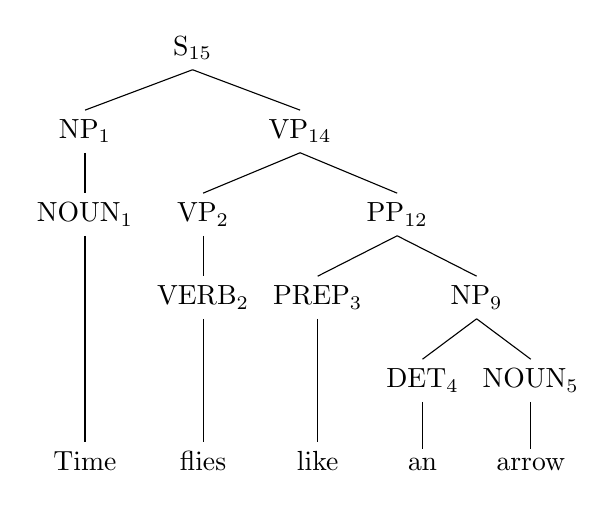
\begin{tikzpicture}
  \tikzset{frontier/.style={distance from root=150pt}}
  \Tree [.$\mathrm{S}_{15}$ [.$\mathrm{NP}_{1}$ [.$\mathrm{NOUN}_{1}$ Time ] ] [.$\mathrm{VP}_{14}$
        [.$\mathrm{VP}_{2}$ [.$\mathrm{VERB}_{2}$ flies ] ] [.$\mathrm{PP}_{12}$ [.$\mathrm{PREP}_{3}$ like ]
        [.$\mathrm{NP}_{9}$ [.$\mathrm{DET}_{4}$ an ] [.$\mathrm{NOUN}_{5}$ arrow ] ] ] ] ]
\end{tikzpicture}

        %}
      }
      \subfloat[time fly(トキバエ?)たちは矢を好む.]{
        \label{fig:tree_flies_2}
        %\resizebox{0.45\linewidth}{!}{
          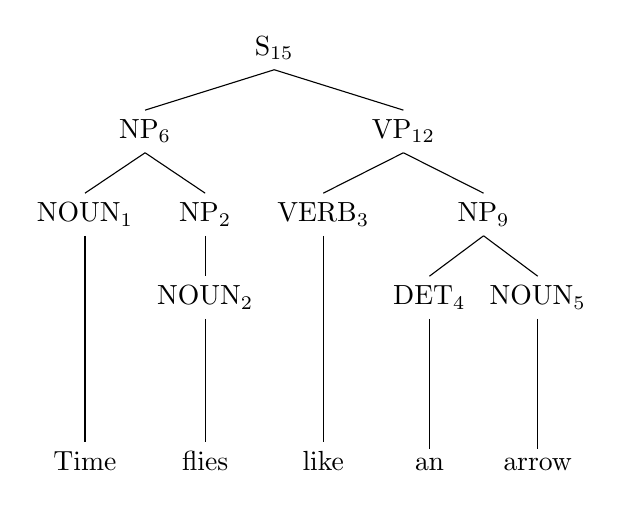
\begin{tikzpicture}
  \tikzset{frontier/.style={distance from root=150pt}}
  \Tree [.$\mathrm{S}_{15}$ [.$\mathrm{NP}_{6}$ [.$\mathrm{NOUN}_{1}$ Time ] [.$\mathrm{NP}_{2}$
        [.$\mathrm{NOUN}_{2}$ flies ] ] ] [.$\mathrm{VP}_{12}$ [.$\mathrm{VERB}_{3}$ like ]
        [.$\mathrm{NP}_{9}$ [.$\mathrm{DET}_{4}$ an ] [.$\mathrm{NOUN}_{5}$ arrow ] ] ] ]
\end{tikzpicture}

        %}
      } \\
      \subfloat[``矢のようなハエ''たちの速度を測定せよ.]{
        \label{fig:tree_flies_3}
        %\resizebox{0.45\linewidth}{!}{
          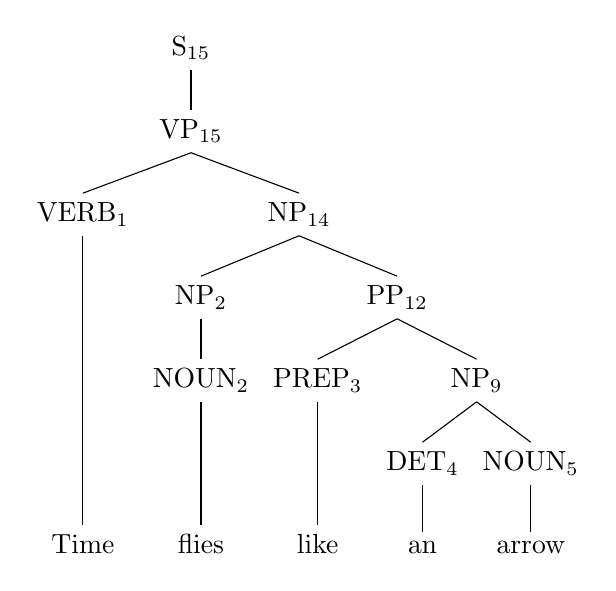
\begin{tikzpicture}
  \tikzset{frontier/.style={distance from root=180pt}}
  \Tree [.$\mathrm{S}_{15}$ [.$\mathrm{VP}_{15}$ [.$\mathrm{VERB}_{1}$ Time ] [.$\mathrm{NP}_{14}$
        [.$\mathrm{NP}_{2}$ [.$\mathrm{NOUN}_{2}$ flies ] ] [.$\mathrm{PP}_{12}$ [.$\mathrm{PREP}_{3}$ like ]
        [.$\mathrm{NP}_{9}$ [.$\mathrm{DET}_{4}$ an ] [.$\mathrm{NOUN}_{5}$ arrow ] ] ] ] ] ]
\end{tikzpicture}

        %}
      }
      \subfloat[矢(の速度を測定するとき)のように,ハエたちの速度を測定せよ.]{
        \label{fig:tree_flies_4}
        %\resizebox{0.45\linewidth}{!}{
          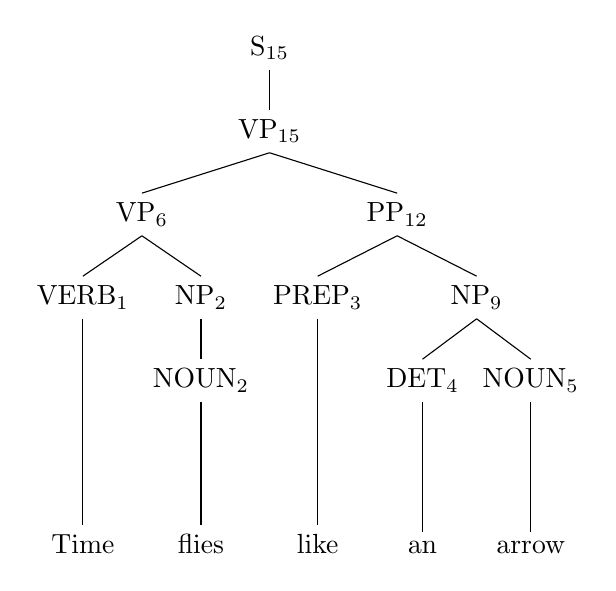
\begin{tikzpicture}
  \tikzset{frontier/.style={distance from root=180pt}}
  \Tree [.$\mathrm{S}_{15}$ [.$\mathrm{VP}_{15}$ [.$\mathrm{VP}_{6}$ [.$\mathrm{VERB}_{1}$ Time ] [.$\mathrm{NP}_{2}$
        [.$\mathrm{NOUN}_{2}$ flies ] ] ] [.$\mathrm{PP}_{12}$ [.$\mathrm{PREP}_{3}$ like ]
        [.$\mathrm{NP}_{9}$ [.$\mathrm{DET}_{4}$ an ] [.$\mathrm{NOUN}_{5}$ arrow ] ] ] ] ]
\end{tikzpicture}

        %}
      }
      \caption{``Time flies like an arrow''の構文木}
      \label{fig:tree_flies}
    \end{figure*}
    \begin{figure*}[htpb]
      \centering
      %\resizebox{0.9\linewidth}{!}{
      \fbox{
        \BVerbatimInput{fig/result_flies.txt}
      }
      \caption{``Time flies like an arrow''のS式(印刷の関係上,出力は改行している.)}
      \label{fig:result_flies}
    \end{figure*}

    実際には,「光陰矢のごとし」以外の候補はいわゆる非文とみなせるが,候補の絞り込みには別の方法を用いる必要性が示唆される.

    \subsection{ネットワーク文法と文脈自由文法の能力の比較}
    \autoref{gaiyou}で触れたように,形式文法は階層構造をなしており,文脈自由文法はネットワーク文法を含む.
    今回作成したプログラムにおいても,CYK法によるpaserを作成する際も,形態素解析の部分にはネットワーク文法のプログラムを流用したことから,これが確認できる.

    ネットワーク文法においても,遷移規則(文法規則)によって簡易的に構文解析ができたが,構文木(S式)まで得るためには文脈自由文法を用いる必要がある.

    しかしながら,文脈自由文法も,今回の考察でも分かったように,文法規則を作成することそのものも困難であるし,複数の構文木が得られてあいまいさが残る問題もある.

    \subsection{実験の感想}
    C言語での実装は比較的大変であったが,オートマトンと構文解析について理解が深まり,本実験の目的は達せられたのではないかと思う.

  \section{まとめ}\label{matome}
  構文解析そのものはプログラムにより実現できたが,構文木が複数得られることから,文の解釈を一意に特定することや非文の生成を防ぐことの困難さが示唆された.

  \bibliography{mybib}
  %\printbibliography[heading=bibintoc, title=文献]
  \flushcolsend

  \onecolumn
  \appendix
  \clearpage
  \section{ネットワーク文法のプログラム}
  \lstinputlisting[caption=Makefile, label=Makefile]{network/Makefile}
  \lstinputlisting[caption=global.h, label=global.h]{network/global.h}
  \lstinputlisting[caption=main.c, label=main.c]{network/main.c}
  \lstinputlisting[caption=dict\_builder.c, label=dict_builder.c]{network/dict_builder.c}
  \lstinputlisting[caption=syntax\_builder.c, label=syntax_builder.c]{network/syntax_builder.c}
  \lstinputlisting[caption=splitter.c, label=splitter.c]{network/splitter.c}
  \lstinputlisting[caption=post.c, label=post.c]{network/post.c}
  \lstinputlisting[caption=network.c, label=network.c]{network/network.c}
  \lstinputlisting[caption=output.c, label=output.c]{network/output.c}
  \begin{figure}[htpb]
    \centering
    \resizebox{.88\linewidth}{!}{
      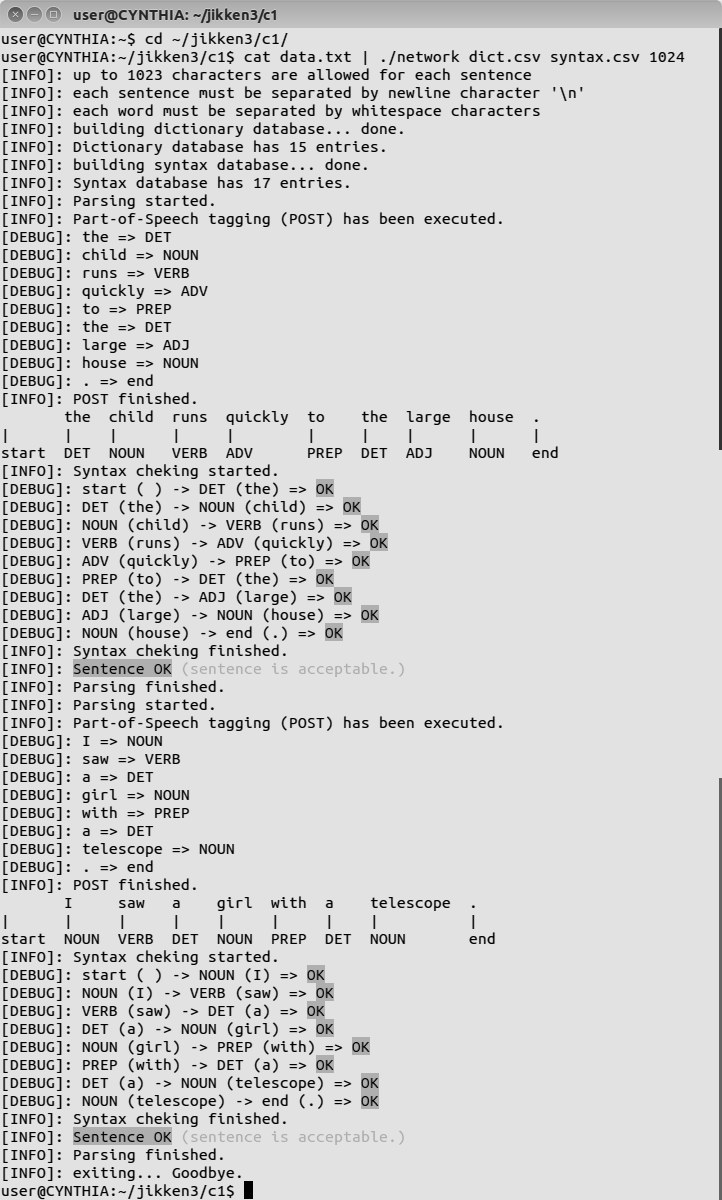
\includegraphics{network/out-mono.png}
    }
    \caption{ネットワーク文法のプログラムの動作風景}
    \label{fig:network}
  \end{figure}

    \subsection{一文の長さの制限変更について}
    初期状態では1文の長さは1023文字に制限されているが,再コンパイルの必要なく,
    第3引数に$n$を渡すことで\(n - 1\)文字までの制限に変更することができる.

    これは文脈自由文法のプログラムにおいても同様である.

  \clearpage
  \section{文脈自由文法のプログラム}
  \lstinputlisting[caption=Makefile, label=Makefile]{cyk/Makefile}
  \lstinputlisting[caption=global.h, label=global.h]{cyk/global.h}
  \lstinputlisting[caption=main.c, label=main.c]{cyk/main.c}
  \lstinputlisting[caption=dict\_builder.c, label=dict_builder.c]{cyk/dict_builder.c}
  \lstinputlisting[caption=syntax\_builder.c, label=syntax_builder.c]{cyk/syntax_builder.c}
  \lstinputlisting[caption=splitter.c, label=splitter.c]{cyk/splitter.c}
  \lstinputlisting[caption=post.c, label=post.c]{cyk/post.c}
  \lstinputlisting[caption=cyk.c, label=cyk.c]{cyk/cyk.c}
  \lstinputlisting[caption=output.c, label=output.c]{cyk/output.c}
  \begin{figure}[htpb]
    \centering
    \resizebox{.88\linewidth}{!}{
      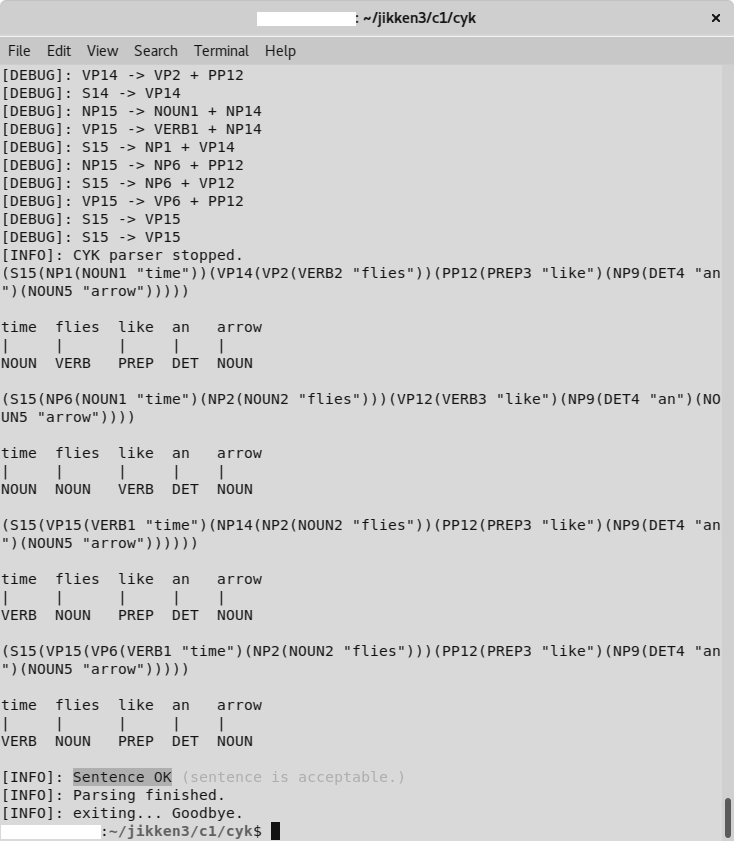
\includegraphics{cyk/out-mono.png}
    }
    \caption{文脈自由文法のプログラムの動作風景}
    \label{fig:network}
  \end{figure}

    \clearpage
    \subsection{インデント機能の使用}
    S式出力用の関数\texttt{print\_sexps}はインデント機能を有している.
    \texttt{main}関数内で
    \begin{equation*}
      \verb|print_sexps(&(cells[CELL_LENGTH - 1].type[i]), type_num, 0);|
    \end{equation*}
    と呼び出している部分の最後の引数を例えば
    \begin{equation*}
      \verb|print_sexps(&(cells[CELL_LENGTH - 1].type[i]), type_num, 4);|
    \end{equation*}
    とすれば4文字でのインデントが有効になり,簡易的に木構造を確認できる(\autoref{fig:result_indent}).

    \begin{figure}[htpb]
      \centering
      %\resizebox{0.9\linewidth}{!}{
      \fbox{
        \BVerbatimInput{fig/result_indent.txt}
      }
      \caption{インデント機能を有効にした場合の出力}
      \label{fig:result_indent}
    \end{figure}
\end{document}
